% Cheatsheet for 01608 and 01609
% Created by Daniel Widerin <daniel@widerin.net>

%\documentclass[8pt,landscape,a4paper]{scrartcl}
\documentclass[9pt,a4paper]{scrartcl}

\usepackage[left=0mm,right=0mm,top=0mm,bottom=5mm]{geometry}
\usepackage{graphicx}
\usepackage[utf8]{inputenc}
\usepackage{multicol}
\usepackage{ngerman}
\usepackage{xcolor}
\usepackage{soul}

% Turn off header and footer
\pagestyle{empty}


% Redefine section commands to use less space
\makeatletter
\renewcommand{\section}{\@startsection{section}{1}{0mm}%
                                {-1ex plus -.5ex minus -.2ex}%
                                {0.5ex plus .2ex}%x
                                {\normalfont\large\bfseries}}
\renewcommand{\subsection}{\@startsection{subsection}{2}{0mm}%
                                {-1explus -.5ex minus -.2ex}%
                                {0.5ex plus .2ex}%
                                {\normalfont\normalsize\bfseries}}
\renewcommand{\subsubsection}{\@startsection{subsubsection}{3}{0mm}%
                                {-1ex plus -.5ex minus -.2ex}%
                                {1ex plus .2ex}%
                                {\normalfont\small\bfseries}}
\renewcommand{\labelitemi}{-}
\makeatother

\newcommand{\compactlist}{\setlength{\itemsep}{-1pt} \setlength{\parskip}{3pt} \setlength{\leftskip}{-1.5em}}

% Don't print section numbers
\setcounter{secnumdepth}{0}
\setlength{\parindent}{0pt}
\setlength{\parskip}{0pt plus 0pt}

\begin{document}

\raggedright
\footnotesize

% put a line between columns
%\setlength{\columnseprule}{0.1pt}

\begin{multicols}{2}

% ------------------------------------------------------------------------------------------------------------------------------
\section{Computersysteme I}

% ------------------------------------------------------------------------------------------------------------------------------
\subsection{Minimalpolynome}
\begin{itemize}
\compactlist
\item{Ein Literal ist ein Ausdruck der Form $X_i^{\epsilon}$ mit $X_i \in V$ und $\epsilon \in \{0,1\}$.}
\item{Ein Monom oder Konjunktionsterm ist ein Ausdruck der Form $\bigwedge_{i\in I} L_i$, wobei die $L_i$ Literale sind für alle $i$ in einer endlichen Indexmenge $I$.}
\item{Ein Polynom oder diskjunktive Normalform(DNF) ist ein Ausdruck der Form $\bigvee_{i\in I} M_i$, wobei die $M_i$ Monome sind für alle $i$ in einer endlichen Indexmenge $I$.}
\item{EIne Klausel oder Disjunktionsterm ist ein Ausdruck der Form $\bigvee_{i\in I} L_i$, wobei die $L_i$ Literale sind für alle $i$ in einer endlichen Indexmenge $I$.}
\item{Eine konjunktive Normalform KNF ist ein Ausdruck der Form $\bigwedge_{i\in I} C_i$, wobei die $C_i$ Klauseln sind für alle $i$ in einer endlichen Indexmenge $I$.}
\item{Alle Minterme sind Monome, alle Maxterme sind Klauseln.}
\item{Alle wesentliche Primimplikaten nennt man auch Kernimplikaten.}
\end{itemize}

% ------------------------------------------------------------------------------------------------------------------------------
\subsection{Schaltnetze}

% ------------------------------------------------------------------------------------------------------------------------------
\subsubsection{Gatter}
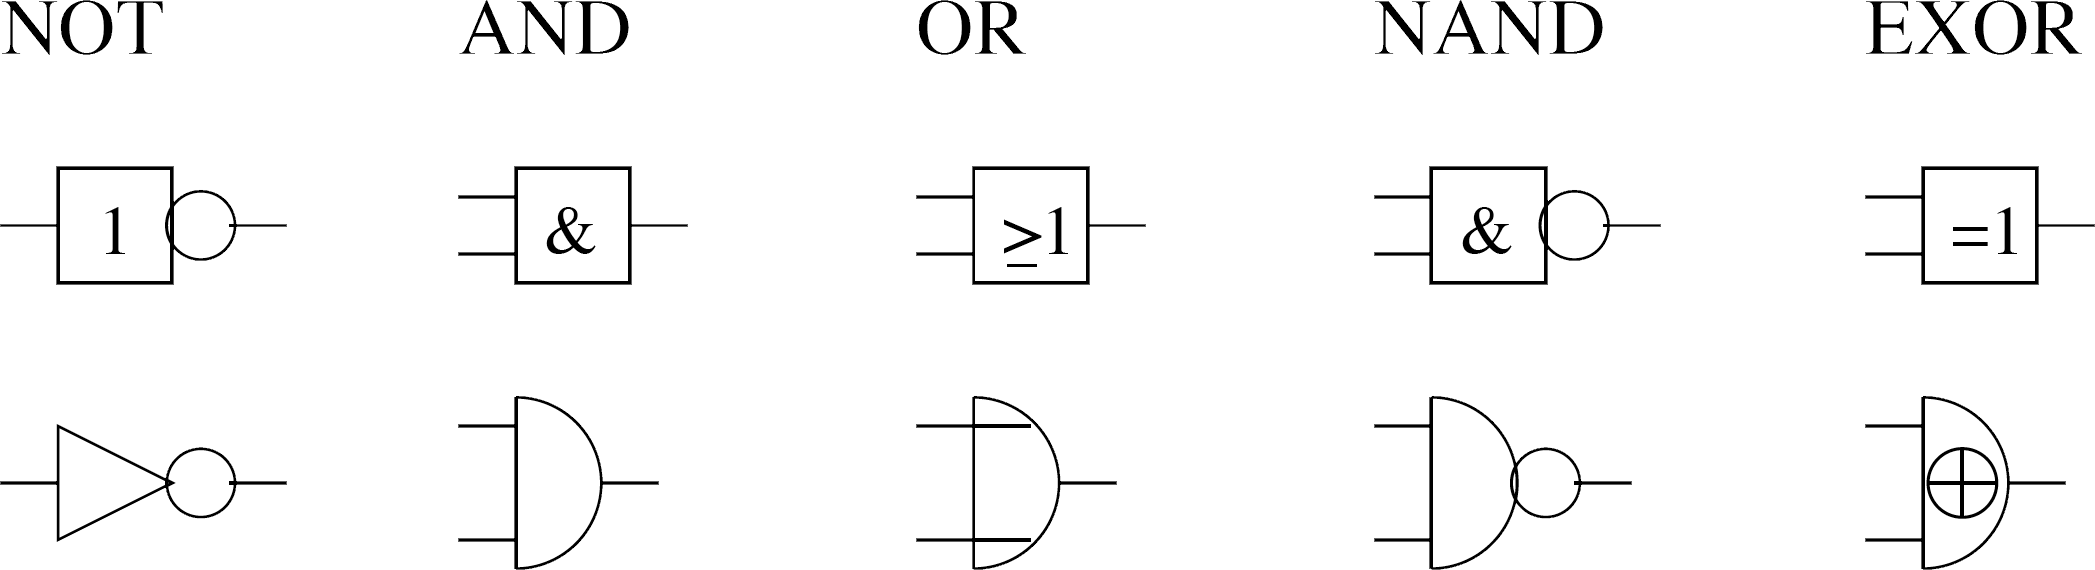
\includegraphics[height=1.75cm]{images/gates.png}

% ------------------------------------------------------------------------------------------------------------------------------
\subsubsection{Komplexitätsmaße}
Satz 2.10: \begin{math}\forall f: \{0,1\}^{n} \rightarrow \{0,1\}\end{math} gilt:\\
\begin{eqnarray}
\nonumber
T(f)\leq C(f) \leq n2^{n}+n
\end{eqnarray}

% ------------------------------------------------------------------------------------------------------------------------------
\subsubsection{Darstellung für ganze Zahlen}
\begin{eqnarray}
\nonumber
\langle a_{n-1}, \ldots, a_0\rangle = &\sum\limits_{i=1}^{n-1} a_i 2^i \Leftrightarrow bin_{n-1}(a)\\
\nonumber
[a_n,a_{n-1}, \ldots, a_0] = &-a_n 2^n + \langle a_{n-1}, \ldots, a_0\rangle \Leftrightarrow twoc_{n}(a)\\
\nonumber
\textnormal{Zweierkomplement}
\end{eqnarray}

% ------------------------------------------------------------------------------------------------------------------------------
\subsubsection{IEEE 754}
\begin{eqnarray}
\nonumber
\langle s|c|a\rangle \Rightarrow &(-1)^s \cdot 1,a \cdot 2^{c-bias}\\
\nonumber
& \begin{tabular}{llll}
SP & bias=127 & m=8 & n=23\\
DP & bias=1023 & m=11& n=52\\
\end{tabular}\\
\nonumber
\end{eqnarray}
\begin{itemize}
\compactlist
\item{Binärzahl berechnen (Bspw.): $34,5_{(10)} = 10 0010,1_{(2)}$}
\item{Exponentenverschiebung (Bspw.): $c = 1,000101\cdot 2^5$}
\item{Exponent berechnen und umrechnen (Bspw.): $c+b = 5+127 = 132_{(10)} = 1000 0100_{(2)}$}
\item{Vorzeichen:  $s = 0|1$}
\end{itemize}

% ------------------------------------------------------------------------------------------------------------------------------
\subsection{Häufig benutzte Schaltnetze}

% ------------------------------------------------------------------------------------------------------------------------------
\subsubsection{Multiplexer}
Ein Multiplexer ist ein Schaltnetz, das mittels des Werts einer Steuerleitung einen von zwei Eingängen auf einen Ausgang weiterleitet. Ein $n$-Bit Multiplexer ($MUX_n$) ist ein Schaltnetz, das die folgende Funktion $m : \{0, 1\}^{2n+1}\rightarrow\{0, 1\}^n$ berechnet.
\begin{eqnarray}
\nonumber
m(a_{n-1}^0, \ldots, a_0^0, a_{n-1}^1, \ldots, a_0^1, s) = \left\{
	\begin{array}{l l l}
	(a_{n-1}^1, \ldots, a_0^1) & \textnormal{falls} & s=1\\
	(a_{n-1}^0, \ldots, a_0^0) & \textnormal{falls} & s=0\\
	\end{array}
	\right.
\end{eqnarray}

Wenn wir für $i = 0,1$ die Abkürzungen $a_i = a_{n-1}^i,\ldots,a_0^i$ vereinbaren, dann können wir die obige Formel auch kürzer schreiben:
\begin{eqnarray}
\nonumber
m(a^0, a^1, s) = a^s
\end{eqnarray}

Es wird gerade der $n$-bit Vektor ausgewählt, dessen oberer Index dem Wert des
Steuersignals $s$ entspricht.
\begin{eqnarray}
\nonumber
T(MUX_n) = &3\\
\nonumber
C(MUX_n) = &3n + 1
\end{eqnarray}

Für $t \geq 2$ ist der $2^t$-Wege $n$-Bit Multiplexer ($MUX_{n,2^t}$) durch die Funktion $m : \{0, 1\}^{2^tn+t}\rightarrow\{0, 1\}^n$ definiert.
\begin{eqnarray}
\nonumber
T(MUX_{n,2^t}) = &2t+1\\
\nonumber
C(MUX_{n,2^t}) = & (2^t-1) \cdot C(MUX_n) \\
\nonumber
= & (2^t-1)\cdot (3n+1)
\end{eqnarray}

% ------------------------------------------------------------------------------------------------------------------------------
\subsubsection{Demultiplexer}
Ein $2$-Wege $n$-Bit Demultiplexer ist ein Schaltnetz zur Berechnung der Funktion $dm : \{0, 1\}^{n+t}  \rightarrow \{0, 1\}^{2^t n}$ mit
\begin{eqnarray}
\nonumber
dm(b, s_{t-1},\ldots , s0) = (a0,\ldots , a^{2t-1})
\end{eqnarray}
wobei
\begin{eqnarray}
\nonumber
a_i = \left\{
	\begin{array}{l l l}
		b & \textnormal{falls} & i=\langle s_{t-1}, \ldots, s_0 \rangle\\
		0 & \textnormal{sonst} & \\
	\end{array}
\right.
\end{eqnarray}

% ------------------------------------------------------------------------------------------------------------------------------
\subsubsection{Coder}
Ein Coder wandelt eine unäre Zahlendarstellung in eine binäre um. Ein $t$-Bit Coder/Encoder ist ein Schaltnetz zur Berechnung der Funktion $cd : \{0,1\}^{2^t} \rightarrow \{0,1\}^{t+2}$ mit
\begin{eqnarray}
\nonumber
cd(a_{2^t-1},\ldots, a_0) = (b_{t+1},\ldots,b_0)
\end{eqnarray}
wobei
\begin{eqnarray}
\nonumber
\langle b_{t-1},\ldots,b_0\rangle = \left\{
	\begin{array}{l l l}
		i & \textnormal{wenn} & a_i=1 \textnormal{ und alle } \\ & & a_j=0 \textnormal{ f\"ur alle } j \not= i\\
		beliebig & \textnormal{sonst} & \\
	\end{array}
\right.
\end{eqnarray}

Im ersten Fall sind $b_{t+1}=b_t=0$. Sind alle $a_i=0$, so ist $b_{t+1}=0$ und $b_t=1$. Sonst ist $b_{t+1}=1$ und der Wert von $b_t$ beliebig.

% ------------------------------------------------------------------------------------------------------------------------------
\subsubsection{Decoder}

Ein Decoder wandelt eine $t$-stellige binäre Zahlendarstellung in eine unäre Zahlendarstellung um. Berechnet wird $dc : \{0,1\}^t \rightarrow \{0,1\}^{2^t}$ mit
\begin{eqnarray}
\nonumber
dc(s_{t-1}, \ldots, s_0) = (a_{2^t-1},\ldots, a_0)
\end{eqnarray}
wobei
\begin{eqnarray}
\nonumber
a_i = \left\{
	\begin{array}{l l l}
		1 & \textnormal{falls} & i=\langle s_{t-1}, \ldots, s_0 \rangle\\
		0 & \textnormal{sonst} & \\
	\end{array}
\right.
\end{eqnarray}

\begin{multicols}{2}

% ------------------------------------------------------------------------------------------------------------------------------
\subsubsection{Arithmetik}
Anzahl Bits Summe bzw. Produkt zweier n-Bit Binärzahlen:\\
n-Bit Binärzahl: \begin{math}0 \leq \langle a\rangle \leq 2^n-1\end{math}\\
\begin{eqnarray}
\nonumber
\langle a\rangle + \langle b\rangle \leq& 2 \cdot (2^n-1) \langle 2^{n+1} \rangle\\
\nonumber
\langle a\rangle \cdot \langle b\rangle \leq& (2^n-1) \cdot (2^n-1)
\end{eqnarray}

% ------------------------------------------------------------------------------------------------------------------------------
\subsubsection{Halb- und Volladdierer}
\begin{eqnarray}
\nonumber
T(HA)=1 & C(HA)=2\\
\nonumber
T(FA)=3 & C(FA)=5
\end{eqnarray}

Volladdierer aus Halbaddierern\vspace{1pt}
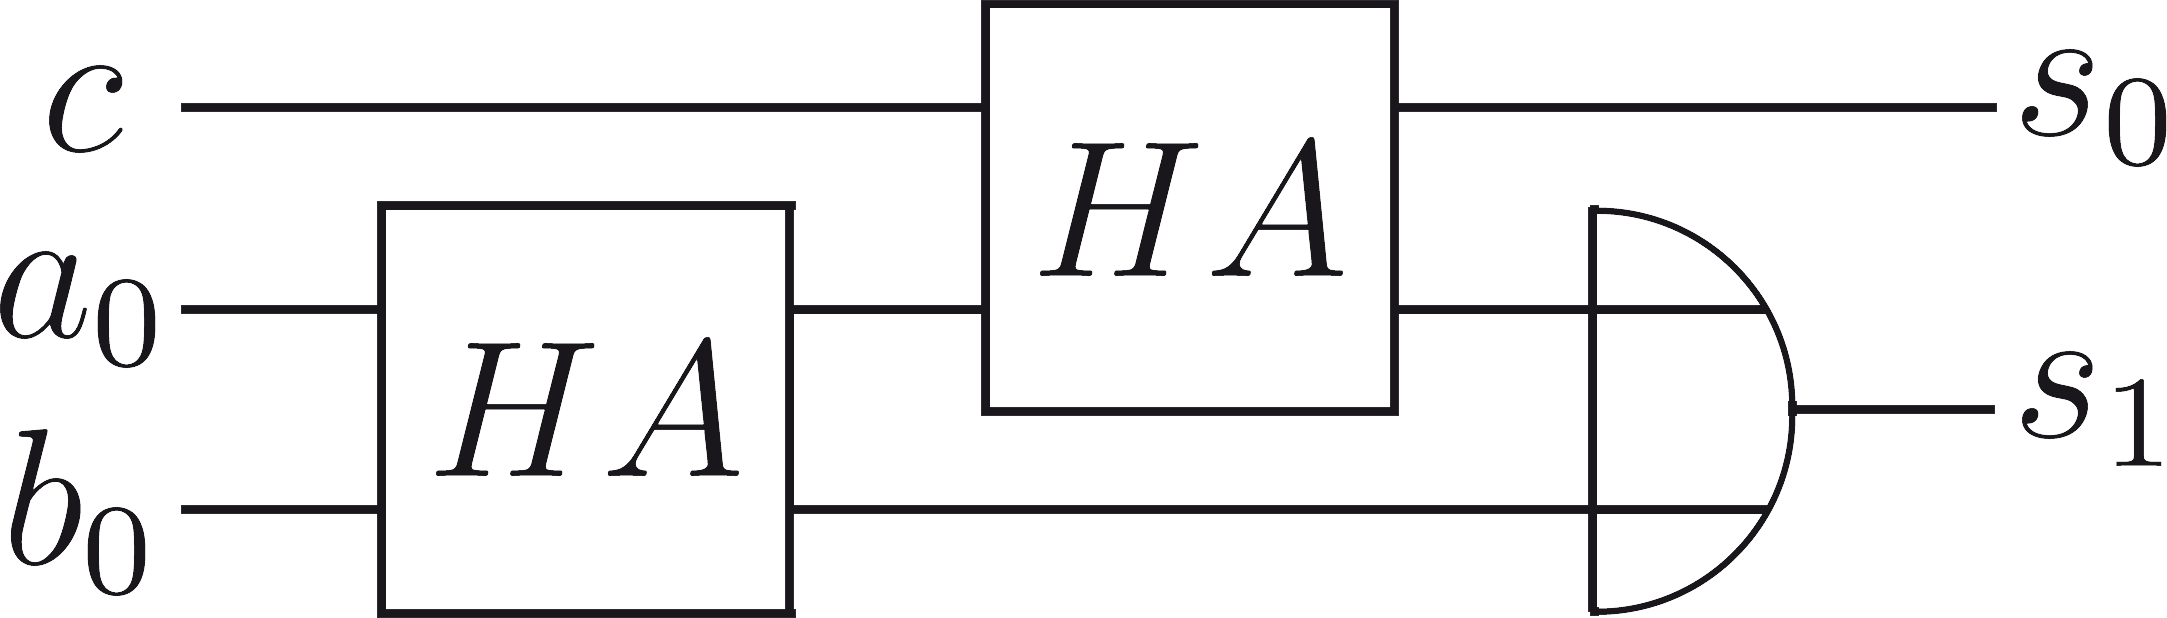
\includegraphics[height=0.75cm]{images/fa-by-ha.png}

% ------------------------------------------------------------------------------------------------------------------------------
\subsubsection{Carry-Chain Addierer}
\begin{eqnarray}
\nonumber
C(A_n) =& n\cdot C(FA) =& 5n\\
\nonumber
T(A_n) \leq& n\cdot T(FA) =& 3n
\end{eqnarray}

\columnbreak
% ------------------------------------------------------------------------------------------------------------------------------
\subsubsection{Conditional Sum Addierer}
Der CS-Addierer hat zwar eine geringe Tiefe dafür aber hohe Kosten.
Für einen $n$-bit Addierer braucht man $3 n/2$-bit Addierer, also $3 \cdot 3 n/4$-bit Addierer usw.

\textbf{Lemma 2.19}: $f(1)=c$ und $f(n) = a \cdot f(n/b) + g(n)$ für $n=b^k$ dann gilt $f(n)=a^{\log_b n}\cdot c+\sum\limits_{i=0}^{\log_b n-1} a^i \cdot g(n/b^i)$

\begin{eqnarray}
\nonumber
C(n) =& 3 \cdot C(n/2)+C(MUX_{n/2+1})\\
\nonumber
T(n) =& T(n/2)+T(MUX_{n/2+1})\\
\nonumber
 \Rightarrow & O(\log n)
\end{eqnarray}

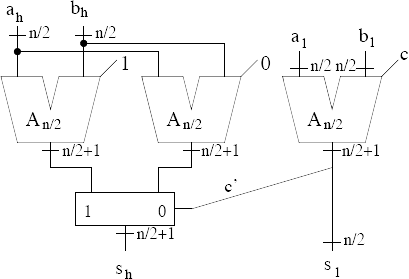
\includegraphics[height=2.5cm]{images/conditional-sum-adder.png}

\end{multicols}

% ------------------------------------------------------------------------------------------------------------------------------
\subsection{Speicherglieder}
\begin{tabular}{ll}
Wirkintervall& $\left\{
\begin{tabular}{ll}

Setup-time&Steuersignals darf sich nicht ändern\\
Hold Time&Dauer die das Steuersignal min. anliegen muss\\
\end{tabular}
\right.$\\
Kippintervall&Ausgänge ändern sich
\end{tabular}
% ------------------------------------------------------------------------------------------------------------------------------
\subsubsection{SR-Latch}

\begin{tabular}{| c | c | c | c || c | c | c | c | c |}
\hline
 &  &  &  &  \multicolumn{4}{c|}{$(t+1)$} & \\
 &  &  &  &  \multicolumn{2}{c}{NOR} & \multicolumn{2}{|c|}{NAND} & \\
$C$ & $S$ & $R$ & $Q(t)$ & $Q$ & $\overline{Q}$ & $Q$ & $\overline{Q}$ & Funktion\\
\hline
0 & X & X & 0 & 0 & 1 & 0 & 1 & speichern\\
0 & X & X & 1 & 1 & 0 & 1 & 0 & speichern\\
1 & 0 & 0 & 0 & 0 & 0 & 0 & 0 & speichern\\
1 & 0 & 0 & 1 & 1 & 0 & 1 & 0 & speichern\\
1 & 1 & 0 & X & 1 & 0 & 1 & 0 & setzen\\
1 & 0 & 1 & X & 0 & 0 & 0 & 0 & rücksetzen\\
1 & 1 & 1 & X & 0 & 0 & 1 & 1 & unzulässig\\
\hline
\end{tabular}

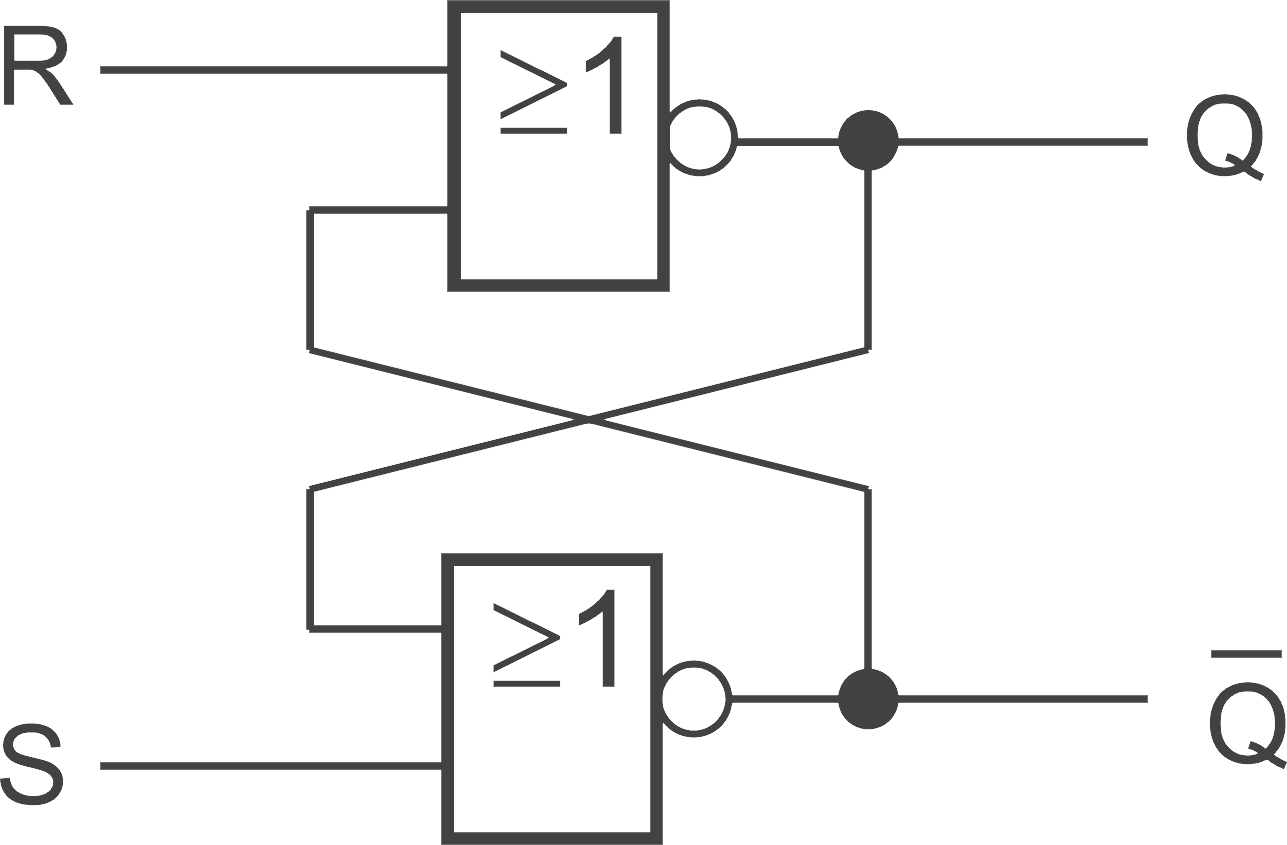
\includegraphics[height=1.5cm]{images/rs-latch-nor.png}
\hspace{0.5cm}
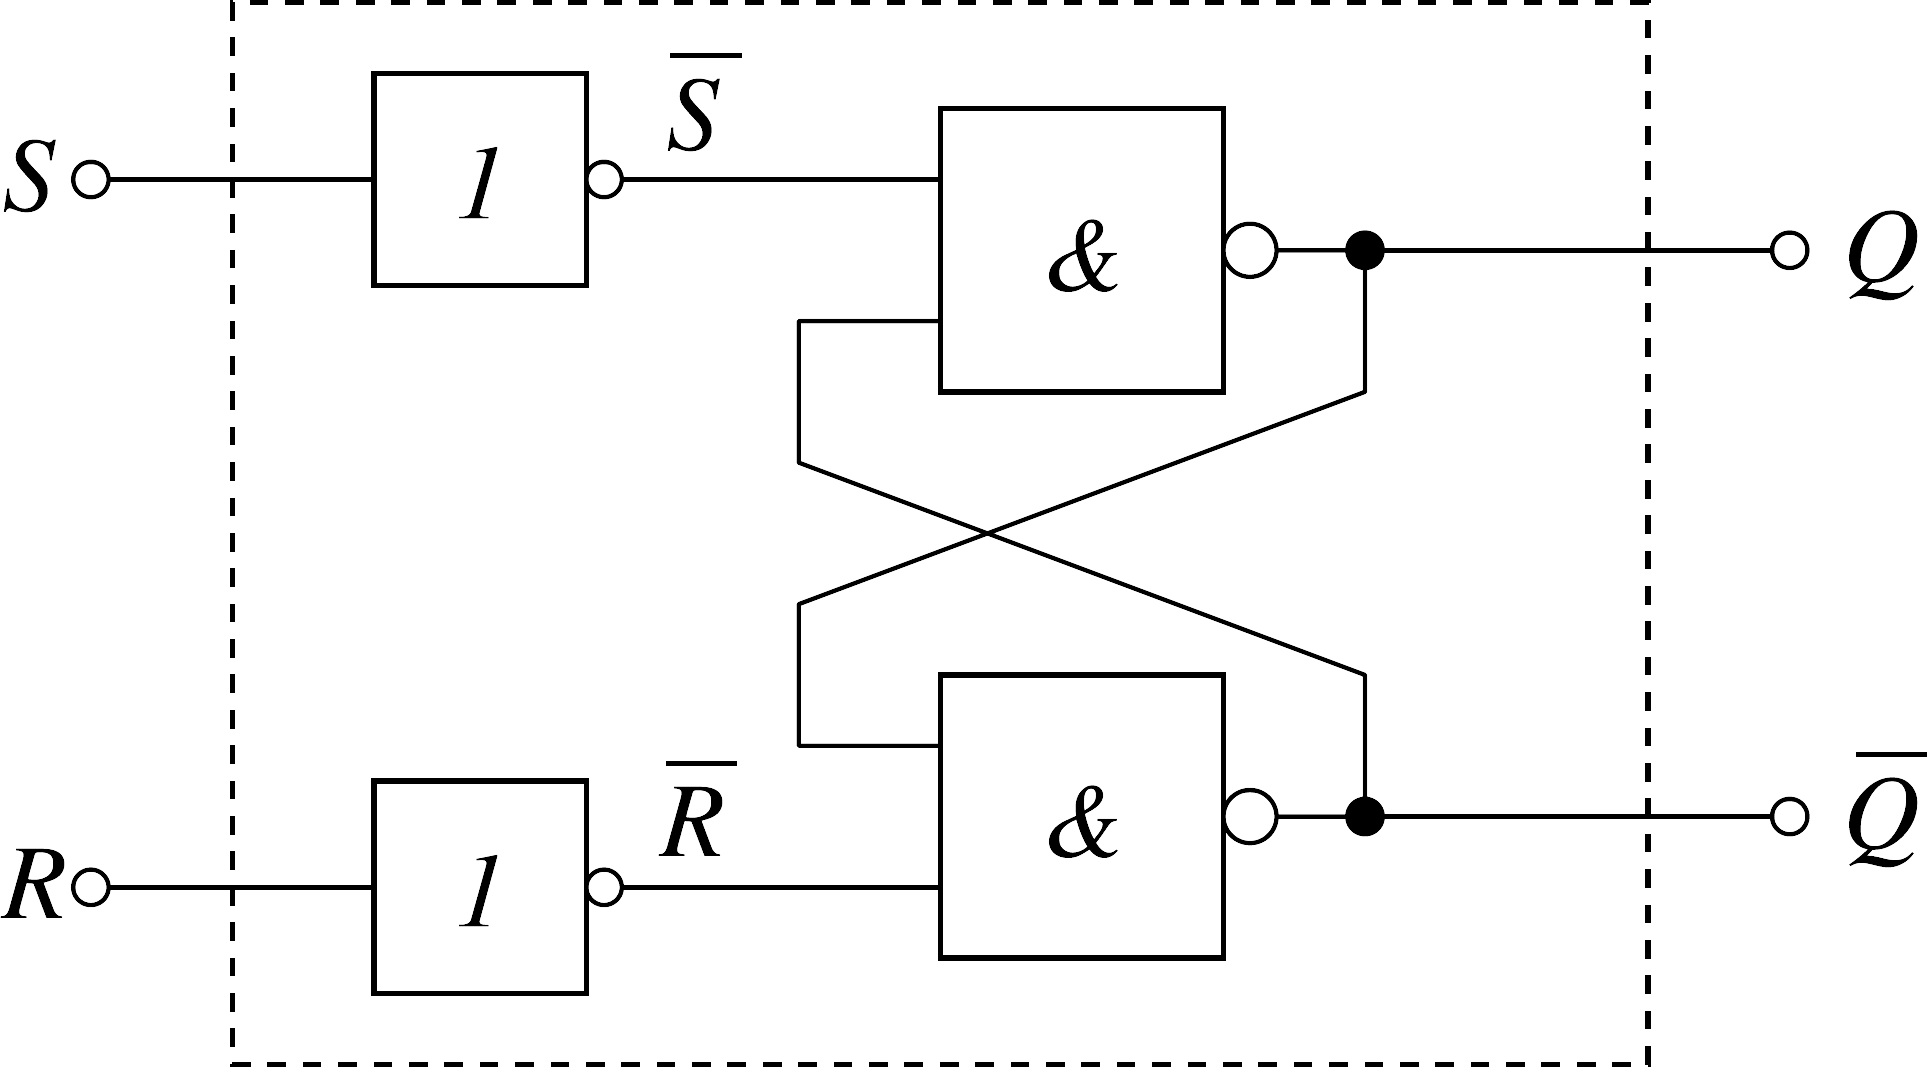
\includegraphics[height=1.5cm]{images/rs-latch-nand.png}

\begin{multicols}{2}

% ------------------------------------------------------------------------------------------------------------------------------
\subsubsection{D-Latch}

\begin{tabular}{ | c | c | c || c |}
\hline
$C$ & $D$ & $Q(t)$ & $Q(t+1)$\\
\hline
0 & X & 0 & 0\\
0 & X & 1 & 1\\
1 & 0 & X & 0\\
1 & 1 & X & 1\\
\hline
\end{tabular}

% ------------------------------------------------------------------------------------------------------------------------------
\subsubsection{JK-FlipFlop}

\begin{tabular}{| c | c | c || c |}
\hline
$J$ & $K$ & $Q(t)$ & $Q(t+1)$\\
\hline
0 & 0 & 0 & 0\\
0 & 0 & 1 & 1\\
0 & 1 & 0 & 0\\
0 & 1 & 1 & 0\\
1 & 0 & 0 & 1\\
1 & 0 & 1 & 1\\
1 & 1 & 0 & 1\\
1 & 1 & 1 & 0\\
\hline
\end{tabular}

% ------------------------------------------------------------------------------------------------------------------------------
\subsection{Umrechnungshilfe}

\begin{tabular}{|c|c|c|}
\hline
\sethlcolor{red}
\hl{$x_{(10)}$} &
\sethlcolor{green}
\hl{$x_{(2)}$} &
\sethlcolor{yellow}
\hl{$x_{(16)}$} \\
\hline
0 & 0000 & 0\\
1 & 0001 & 1\\
2 & 0010 & 2\\
3 & 0011 & 3\\
\hline
4 & 0100 & 4\\
5 & 0101 & 5\\
6 & 0110 & 6\\
7 & 0111 & 7\\
\hline
8 & 1000 & 8\\
9 & 1001 & 9\\
10 & 1010 & A\\
11 & 1011 & B\\
\hline
12 & 1100 & C\\
13 & 1101 & D\\
14 & 1110 & E\\
15 & 1111 & F\\
\hline
\end{tabular}

\end{multicols}

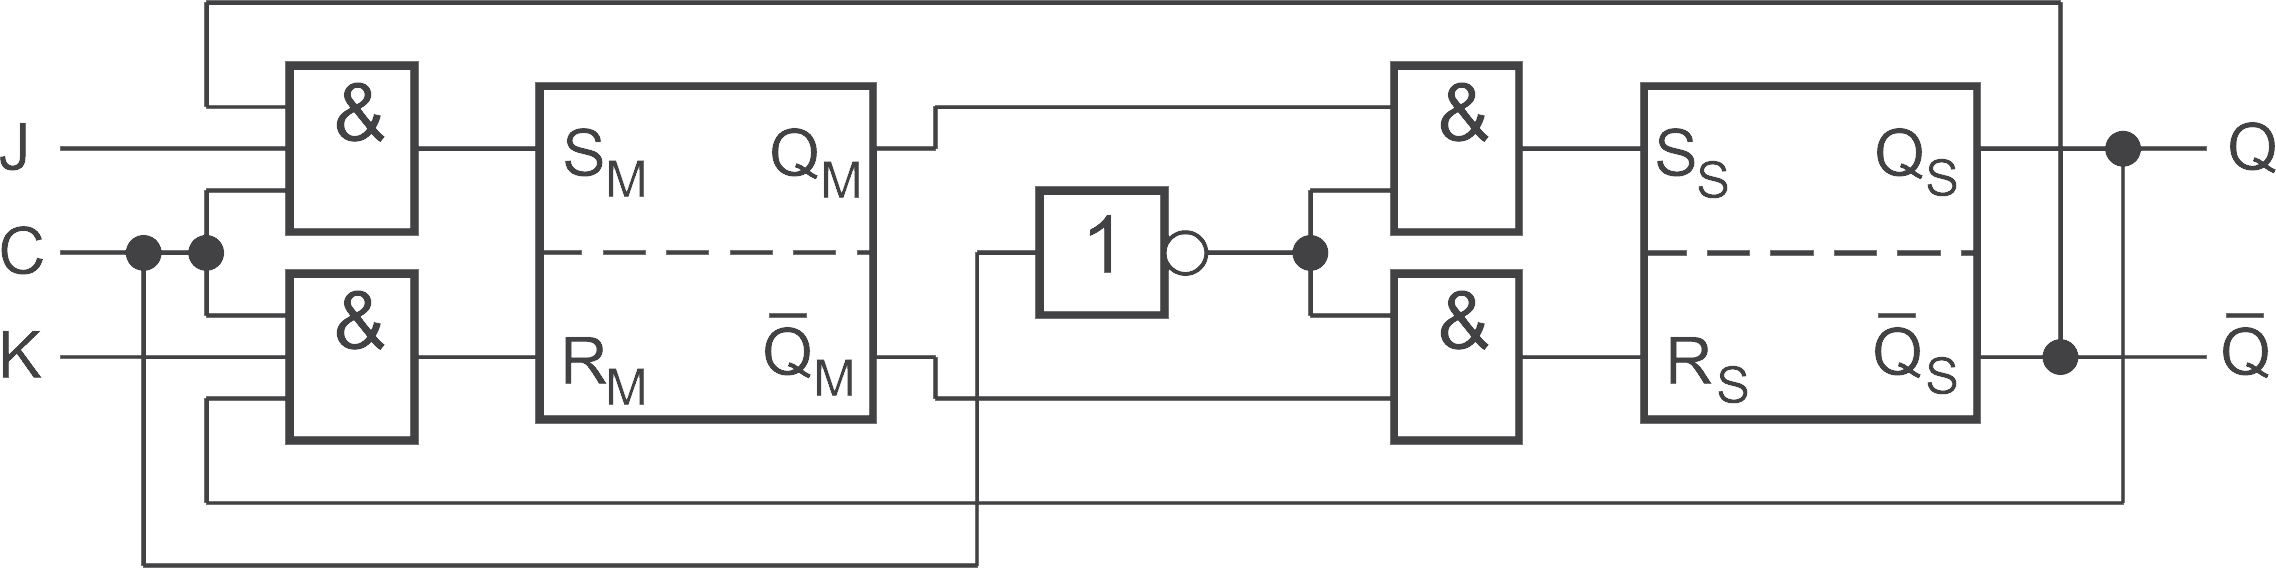
\includegraphics[height=1.5cm]{images/jk-ff.png}

% ------------------------------------------------------------------------------------------------------------------------------
\subsection{Programmierbare Logikbausteine}

\begin{tabular}{ | l | c | c | }
\hline
Art & AND-Matrix & OR-Matrix\\
\hline
ROM & fest & fest\\
PROM, EPROM, EEPROM & fest & programmierbar\\
PAL & programmierbar & fest\\
PLA & programmierbar & programmierbar\\
\hline
\end{tabular}

% ------------------------------------------------------------------------------------------------------------------------------
\subsection{ASM-Regeln}
\begin{enumerate}
\compactlist
\item{Pfade durch die Entscheidungsboxen führen genau zu einem Zustand.}
\item{Variablen in der Zustandsbox oder in bedingten Ausführungsboxen dürfen innerhalb eines ASM-Blocks nur einmal auf der linken Seite stehen, d.h. sie dürfen nur eimal pro Taktzyklus beschrieben werden.}
\item{Die Wertezuweisung an die Variablen erfolgen erst am Ende eines Taktzyklus, d.h. innerhalb des Zustandes werden auf der rechten Seite von Zuweisungen und in Entscheidungsboxen die Werte benutzt, die die Variablen am Anfang des Zustands haben. Die im Zustand neu zugewiesenen Werte sind also erst kurz nach Ende des Taktzyklus (am Anfang des Folgezustands) gültig.}
\end{enumerate}

\pagebreak

% ------------------------------------------------------------------------------------------------------------------------------
\section{Computersysteme II}

% ------------------------------------------------------------------------------------------------------------------------------
\subsection{Befehlssatzarchitekturen}

\textbf{Prozessorarchitektur} (Befehlssatzarchitektur, Programmiermodell, ISA) definiert die Grenze zw. Hard- und Software und beinhaltet keine Details der Hardware und der technischen Ausführung des Prozessors nur äußeres Erscheinungsbild mit (Befehlssatz, Befehlsformat, Adressierungsarten, System der Unterbrechungen, Speichermodell (Register und Adressraumaufbau)

\vspace{0.5em}
\textbf{Mikroarchitektur}: bezeichnet die Hardware-Struktur und der Entwurf der Kontroll- und Datenpfad (Art und Stufen der Pipeline, Superskalartechnik, Ausführungseinheiten, Primär Cache Speicher.

% ------------------------------------------------------------------------------------------------------------------------------
\subsubsection{Adressraumorganisation}
\textbf{Architekturregister} ist der Überbegriff für die Register welche in der Architektur sichtbar sind. (\textbf{nicht} physikalische Register oder Umbenennungspufferregister).

\vspace{0.5em}
\textbf{Big-endian}-Format \emph{(most significant byte first)} speichert von links nach rechts; \textbf{Little-endian}-Format \emph{(least significant byte first)} von rechts nach links.

% ------------------------------------------------------------------------------------------------------------------------------
\subsubsection{Befehlsformate}
\begin{itemize}
\compactlist
\item{\textbf{Dreiadressformat}: \begin{tabular}{ |c|c|c|c| }
\hline
Opcode&Dest&Src1&Src2\\
\hline
\end{tabular}}
\item{\textbf{Zweiadressformat}: \begin{tabular}{ |c|c|c| }
\hline
Opcode&Dest/Src1&Src2\\
\hline
\end{tabular}}
\item{\textbf{Einadressformat}: \begin{tabular}{ |c|c| }
\hline
Opcode&Src\\
\hline
\end{tabular} (Wert auf Akkumulatorregister)}
\item{\textbf{Nulladressformat}: \begin{tabular}{ |c| }
\hline
Opcode\\
\hline
\end{tabular} (benötigt Stackarchitektur)}
\end{itemize}

% ------------------------------------------------------------------------------------------------------------------------------
\subsubsection{Adressierungsarten}
MMU rechnet effektive Adresse in physikalische (=Adresse im HSP) um.
\begin{itemize}
\compactlist
\item{\textbf{Register direkt} (\emph{register}): Operand steht im Register}
\item{\textbf{Register indirekt} (\emph{register indirect}): Operandenadresse steht in Register}
\item{\textbf{unmittelbare} (\emph{immediate}): Operand steht als Konst.}
\item{\textbf{direkte/absolute} (\emph{absolute}): Operandenadresse}
\end{itemize}
Spezialfälle
\begin{itemize}
\compactlist
\item{\textbf{Register indirekt mit Autoinkrement/-dekrement} (\emph{autoincrement/autodecrement}): (wie Register indirekt aber mit inkr./dekr., vorallem für Schleifen)}
\item{\textbf{indizierte} (\emph{indirect indexed}): Summe aus Registern}
\item{\textbf{indizierte mit Verschiebung} (\emph{indirect indexed with displacement}): Summe aus Registern + Verschiebung im Befehlswort}
\item{\textbf{befehlszählerrelativ} (\emph{PC-relative}): PC+4}
\item{\textbf{befehlszählerindirekt} (\emph{PC-indirect}): Register als Zeiger auf Speicheradresse bei dem der Programmablauf fortgefahren wird.}
\end{itemize}

% ------------------------------------------------------------------------------------------------------------------------------
\subsubsection{RISC \textnormal{(\textbf{R}educed \textbf{I}nstruction \textbf{S}et \textbf{C}omputers)}}
\begin{itemize}
\compactlist
\item{kleiner Befehlssatz, wenige, nur notwendige Befehle u. Adressierungsarten}
\item{große Registerzahl (Voraussetzung: billige Speichertechnologie)}
\item{Laden und Speichern erfolgt nur über LOAD/STORE Befehle}
\end{itemize}

% ------------------------------------------------------------------------------------------------------------------------------
\subsubsection{CISC \textnormal{(\textbf{C}omplex \textbf{I}nstruction \textbf{S}et \textbf{C}omputers)}}
\begin{itemize}
\compactlist
\item{Hohe Codedichte}
\end{itemize}

% ------------------------------------------------------------------------------------------------------------------------------
\subsection{Pipeline}

\begin{tabular}{ | c | c | c | c | c | }
\hline
IF & ID & EX & MEM & WB\\
\hline
\end{tabular}
\begin{tabular}{ll}
IF & \textbf{I}nstruction \textbf{F}etch\\
ID & \textbf{I}nstruction \textbf{D}ecode\\
EX & \textbf{Ex}ecute / Address Calculation\\
MEM & \textbf{Mem}ory Access (wird nur f\"ur \\
 & Lade/Speichern und bedingte\\
 & Spr\"unge ben\"otigt.\\
WB & \textbf{W}rite \textbf{B}ack\\
\end{tabular}\\
\vspace{2mm}
Beschleunigung (Speedup S) von $n$ Befehlen in $k$ Takten ist definiert durch:
\begin{eqnarray}
\nonumber
S=\frac{n \cdot k}{k+n-1}=\frac{k}{k/n+1-1/n}
\end{eqnarray}

% ------------------------------------------------------------------------------------------------------------------------------
\subsubsection{Pipelinekonflikte}
\begin{itemize}
\compactlist
\item{\textbf{Datenkonflikte}: Operand steht nicht zur Verfügung.}
\item{\textbf{Steuerflusskonflikte}: Zieladresse des als nächstes auszuführenden Befehls ist noch nicht bekannt.}
\item{\textbf{Stuktur- oder Resourcenkonflikte}: }
\end{itemize}

% ------------------------------------------------------------------------------------------------------------------------------
\subsubsection{Datenunabh\"angigkeit / Datenkonflikte}
\begin{itemize}
\compactlist
\item{echte Datenabhängigkeit (true dependency)\\RAW (read after write)}
\item{Gegenabhängigkeit (anti dependency)\\WAR (write after read)}
\item{Ausgabeabhängigkeit (output dependency)\\WAW (write after write)}
\end{itemize}

% ------------------------------------------------------------------------------------------------------------------------------
\subsubsection{Sprünge}

\begin{tabular}{lll}
BTAC & \emph{Branch-target Address Cache} & Sprungzieladress-Cache\\
BTB & \emph{Branch-target Buffer} & Sprungzielpuffer
\end{tabular}

% ------------------------------------------------------------------------------------------------------------------------------
\subsubsection{VLIW \textnormal{(\textbf{V}ery \textbf{L}ong \textbf{I}nstruction \textbf{W}ord)}}
\begin{itemize}
\compactlist
\item{ist eine Architekturtechnik bei der ein Compiler mehrere von einander unabhängige Befehle zu einem Befehlswort (meist fester Länge) zusammenpackt}
\item{Ist angewiesen auf eine statische (durch den Compiler definierte) Befehlsanordnung}
\item{dadurch geringere Hardwarekomplexität als bei normaler Superskalartechnik}
\end{itemize}

% ------------------------------------------------------------------------------------------------------------------------------
\subsubsection{EPIC  \textnormal{(\textbf{E}xplicit \textbf{P}arallel \textbf{I}nstruction \textbf{C}omputing)}}
\begin{itemize}
\compactlist
\item{bezeichnet das (Drei-)Befehlsformat des IA-64-Befehlssatzes, ähnlich dem dreifach VLIW Format}
\item{Versucht die Vorteile der hohen VLIW-Taktrate mit dynamischen Scheduling zu verbinden}
\item{prädikativ}
\end{itemize}

% ------------------------------------------------------------------------------------------------------------------------------
\subsection{Superskalartechnik}
\ldots ist eine Mikroarchitektur und hat keinen Einfluss auf die Befehlssatzarchitektur! Sie nutzt die \textbf{feinkörnige Parallelität}, d.h. Parallelität zwischen einzelnen Befehlen. Pipelining nutzt \textbf{zeitliche}, die Superskalartechnik die \textbf{räumliche Parallelität} aus.

\begin{itemize}
\compactlist
\item{mehr als ein Befehl pro Takt}
\item{hardwareseitige dynamische Bestimmung der Anzahl der zugewiesenen Befehle pro Takt}
\item{sequenzieller Strom von normalen Befehlen}
\end{itemize}

VLIW und EPIC sind Architekturtechniken, wohingegen die Superskalartechnik eine Mikroarchitekturtechnik ist!

% ------------------------------------------------------------------------------------------------------------------------------
\subsubsection{Code-Cache-Speicher}
wird in der IF-Stufe mit dem nächsten Befehlsblock - der mindestens der Zuordnungsbandbreite des Superskalarprozessors entspricht - gefüllt, um die Pipeline mit Befehlen zu versorgen. Durch eine \textbf{Harvard-Cache-Architektur} (eigener Code- und Daten-Cache-Speicher) kann in jedem Takt solch ein Block bereitgestellt werden.

% ------------------------------------------------------------------------------------------------------------------------------
\subsubsection{Sprungvorhersagetechniken}
Um eine effiziente Sprungbehandlung zu erzielen muss
\begin{itemize}
\compactlist
\item{Sprungrichtung muss möglichst früh bekannt sein}
\item{Sprungzieladresse muss im Sprungzieladress-Cache (BTAC) nach erstmaligem Berechnen gespeichert sein und sofort in den PC geladen werden}
\item{Möglichst genaue Vorhersage der Sprünge}
\item{Mehrere Ebenen der Spekulation müssen unterstützt werden}
\item{Bei falscher Vorhersage muss schnell zurückgerollt werden können}
\end{itemize}

Test kann bis in die ID Stufe vorgezogen werden, können statisch (z.b. \emph{always taken}) und/oder dynamisch implementiert werden:

\begin{itemize}
\compactlist
\item{\textbf{Ein-Bit-Prädiktor} speichert NT/T in einem Bit; implementiert in der IF-Stufe, benötigt BHT}
\item{\textbf{Zwei-Bit-Prädiktor} speichert ST//WT/WNT/SNT, kann mit Sättigungszähler oder Hysteresezähler implementiert werden.}
\item{\textbf{Korrelationsprädiktoren} brücksichtigt neben Vergangenheit auch die Historie benachbarter Sprünge. ($m,n$)-Prädiktor nutzt das Verhalten der letzten $m$ Sprünge um $2^m$ Prädiktoren auszuwählen. ($n=2$ für Zwei-Bit-Prädiktor). Sprungverlaufsregister BHR (\emph{Branch History Register}) wählt eintrag aus Sprungverlaufstabelle PHT (\emph{Pattern History Table}}
\item{\textbf{Prädikation} ermöglicht durch Prädikatbits im Befehl beide Sprungrichtungen auszuführen und die falsche zu verwerfen. Beeinflusst Architektur durch zusätzliche Befehle im Befehlssatz und erhöht Komplexität der Mikroarchitektur. (Bsp: IA-64)}
\item{\textbf{Mehrpfadausführung} führt ebenfalls beide Sprungrichtungen aus und verwirft die falsche, jedoch ohne Prädikatbits und neuen Befehlen, somit eine Mikroarchitekturtechnik. Selten implementiert, hoher Resourcenverbrauch}
\end{itemize}

% ------------------------------------------------------------------------------------------------------------------------------
\subsubsection{Registerumbenennung}
\begin{itemize}
\compactlist
\item{...beseitigt scheinbare Datenabhängigkeit (Gegenabhängigkeiten und Ausgabeabhängigkeiten) zwischen Registeroperanden.}
\item{Ohne Registerumbenennung könnten Ausgabeabhängigkeiten das Ergebnis verfälschen.}
\item{kann statisch (Compilertechnik) oder dynamisch (Hadware, Mikroarchitekturtechnik) erfolgen}
\item{kann als Alternative z.b. statisch und - wie beim IA-64 - mit roßem Registersatz verwendet werden.}
\end{itemize}

% ------------------------------------------------------------------------------------------------------------------------------
\subsubsection{Befehlszuordnung}
\begin{itemize}
\compactlist
\item{\textbf{Befehlsfenster} entkoppelt den Befehlsbereitstellungs- und Decodierteil vom Ausführungsteil des Prozessors. Befehle im -fenster sind durch \textbf{Sprungvorhersagen} frei von Steuerflussabhängigkeiten und durch die \textbf{Registerumbenennung} frei von Namensabhängigkeiten}
\item{dynamische Befehlszuordnung der Superskalarprozessoren kann mit einem statischen Scheduling (vom Compiler) oder mit einem dynamischen Scheduling verknüpft werden}
\item{um die Ausführungseinheiten optimal zu nutzen, müssen in jedem Takt die Verfügbarkeit aller Eingabeoperanden eines Befehls und Verfügbarkeit der Ressourcen geprüft, ausführbereite Befehle selektiert und zugeordnet werden}
\item{Ergebnisse werden in temporären Registern abgelegt}
\item{SIMD \textbf{S}ingle \textbf{I}nstruction \textbf{M}ultiple \textbf{D}ata d.h. Operationen sind gleichartig}
\end{itemize}

% ------------------------------------------------------------------------------------------------------------------------------
\subsection{Speicherverwaltung}

Gesamtanzahl der Blockrahmen $c$ in einem Cache-Speicher enspricht dem Produkt aus der Anzahl $s$ der Sätze und der Assoziativität $n$, also $c = s \cdot n$

\begin{tabular}{llll}
DM & direkt abgebildet & $s=c, n=1$ & vgl. Index und Tag\\
An & $n$-fach satzassoziativ & $s=c/n$ & vgl. Index und Tag\\
AV & vollassozialtiv & $s=1, n=c$ & vgl. Tag\\
\end{tabular}

\begin{tabular}{llll}
Wortbits & Blockgröße = $2^{\#r} \Rightarrow \#r=\ldots$\\
Indexbits & s = $2^{\#q} \Rightarrow \#q=\ldots$\\
\end{tabular}

Cache-$Hit$ wenn im aktuellen Index das Tag übereinstimmt, sonst $Miss$

Mesi benötigt 2 zusätzliche Bits:
\begin{tabular}{ll}
M & exclusive \textbf{M}odified\\
E & \textbf{E}xclusive unmodified\\
S & \textbf{S}hared unmodified\\
I & \textbf{I}nvalid\\
\end{tabular}

% ------------------------------------------------------------------------------------------------------------------------------
\subsection{Parallele Systeme}

\begin{tabular}{ll}
$T=$ & $T_{comm}+T_{comm}+T_{idle}$\\
$T_{comp}$ & Berechnungszeit \emph{(computation time)}\\
$T_{comm}$ & Kommunikationszeit \emph{(communication time)}\\
$T_{idle}$ & Untätigkeitszeit \emph{(idle time)}\\
$T(1) = P(1)$ &  eine Operation/Schritt auf einem Prozessor\\
$T(n) \leq P(n)$ & mehr Operationen/Schritt auf $n$ Prozessoren\\
$S(n)=\frac{T(1)}{T(n)}$ & Beschleunigung \emph{(Speed-up)} wobei $1 \leq S(n)\leq n$\\
$E(n)=\frac{S(n)}{n}$ & Effizienz (efficiency) wobei $\frac{1}{n}\leq E(n) \leq 1$\\
$R(n)=\frac{P(n)}{P(1)}$ & Mehraufwand für die Parallelisierung\\
$I(n)=\frac{P(n)}{T(n)}$ & Parallelindex \emph{(parallel index)}\\
$U(n)=\frac{I(n)}{n}$ & $=R(n)\cdot E(n)$: Auslastung \emph{(utilization)} \\
$T(n)=$ & $T(1)\cdot\frac{1-a}{n}+T(1) \cdot a$\\
$S(n)=$ & $\frac{T(1)}{T(1)\cdot \frac{1-a}{n} + T(1) \cdot a}=\frac{1}{\frac{1-a}{n}+a}$\\
\end{tabular}

\end{multicols}

\end{document}
